\chapter{Background}
\label{ch:background}
Our ideas and implementation are based on dependent type theory (DTT). It is the meta theory for this work. We introduce it in Section~\ref{subsec:background:dtt} and define the notion of a theory and a context in Section~\ref{sec:background:theory}.
% Equational logic is based in set theory and forms the bases for universal algbera.  Dependent type theory (DTT) is a rich type theory in which types can depend on values. We want to represent theories of equational logic as contexts in DTT. We first introduce equational logic and DTT in Section~\ref{sec:background:logic}. 
%Contexts are defined in Section~\ref{sec:background:context} and theories in Section~\ref{sec:background:theory}. We then briefly introduce universal algebra and how it is used in our work in Section~\ref{sec:background:ualgebra}. 

Part of our work is building a library of axiomatic theories. The library is organized as a theory graph, in which theories are connected via morphisms. We introduce morphisms in Section~\ref{sec:background:morphisms} and discuss theory graphs and different strategies for building them in Section~\ref{sec:background:theorygraph}. 
To build the library we use combinators motivated by category theory, so we give a brief introduction for that in Section~\ref{sec:categoryTh}. 
Two of the constructions we generate are not typically defined within universal algebra texts. These are relational interpretations and staged terms, used in multi-staged programming. We give details on these in Sections~\ref{sec:background:relInterp} and~\ref{sec:background:msp}, respectively. 

\section{Dependent Type Theory}
\label{subsec:background:dtt}
Dependent type theory (DTT) is a version of type theory that enables writing types like 
\lstmath{$\Pi\ $ x : A $\ \cdot\ $ M x}, % \text{x : A} \cdot \text{M x}$} % x : A $\ \cdot\ $ M x} 
where the type \lstmath{M x} depends on the \emph{value} of \lstmath{x}, i.e. \lstmath{M : A $\ \to\ $ Type}. 
% source: Type theory and formal proof, P. 103 - Ch.5 
Having types that depend on values adds to the expressiveness of the logic. A common example for introducing dependent types is the type of a vector of \lstmath{n} elements of a type \lstmath{A}. 
In most programming languages, the type of this vector is defined in terms of the type of its elements as \lstmath{Vec A}. Using dependent types, the type of a vector can depend on both the type of its elements and also its length, written as \lstmath{$\Pi\ $ n : $\ \mathbb{N}\ \cdot\ $ Vec A n}.
 
Having this extra information in the type allows detection of some errors, like accessing out of bounds elements, during type checking. 

DTT is seen by many as a convenient foundation for representing mathematics~\cite{whyDttCoq, whyDTTbauer, nCatShulman}. It lets one express ideas frequently used in mathematics. Statements like "the non-zero element", operations such as projecting the first unit vector in a specific dimension, or representation of a family of sets. 
The constructive nature of DTT adds the advantage that proofs can be run as programs. 
%,  the specification is the type of the function 
%The descriptive power of DTT makes it more suitable for capturing mathematical knowledge. Therefore, many of the modern mechanized mathematics systems use variants of DTT as their foundations.\ednote{check this}  

Figures~\ref{fig:dttGrammar} and~\ref{fig:dtt-w-sigma} shows the grammar and typing rules of a small version of dependent type theory with $\Pi$- and $\Sigma$-types like the one we use. The terms permissible in this type theory are variables, $\lambda$-abstractions, function applications, dependent type pairs, and their projections. 
%In additions to types and type applications, the DTT we present here allows $\Pi$- and $\Sigma$-types. The concepts of $\Sigma$-types and contexts will be discussed shortly in this section.

\begin{figure}
\centering{
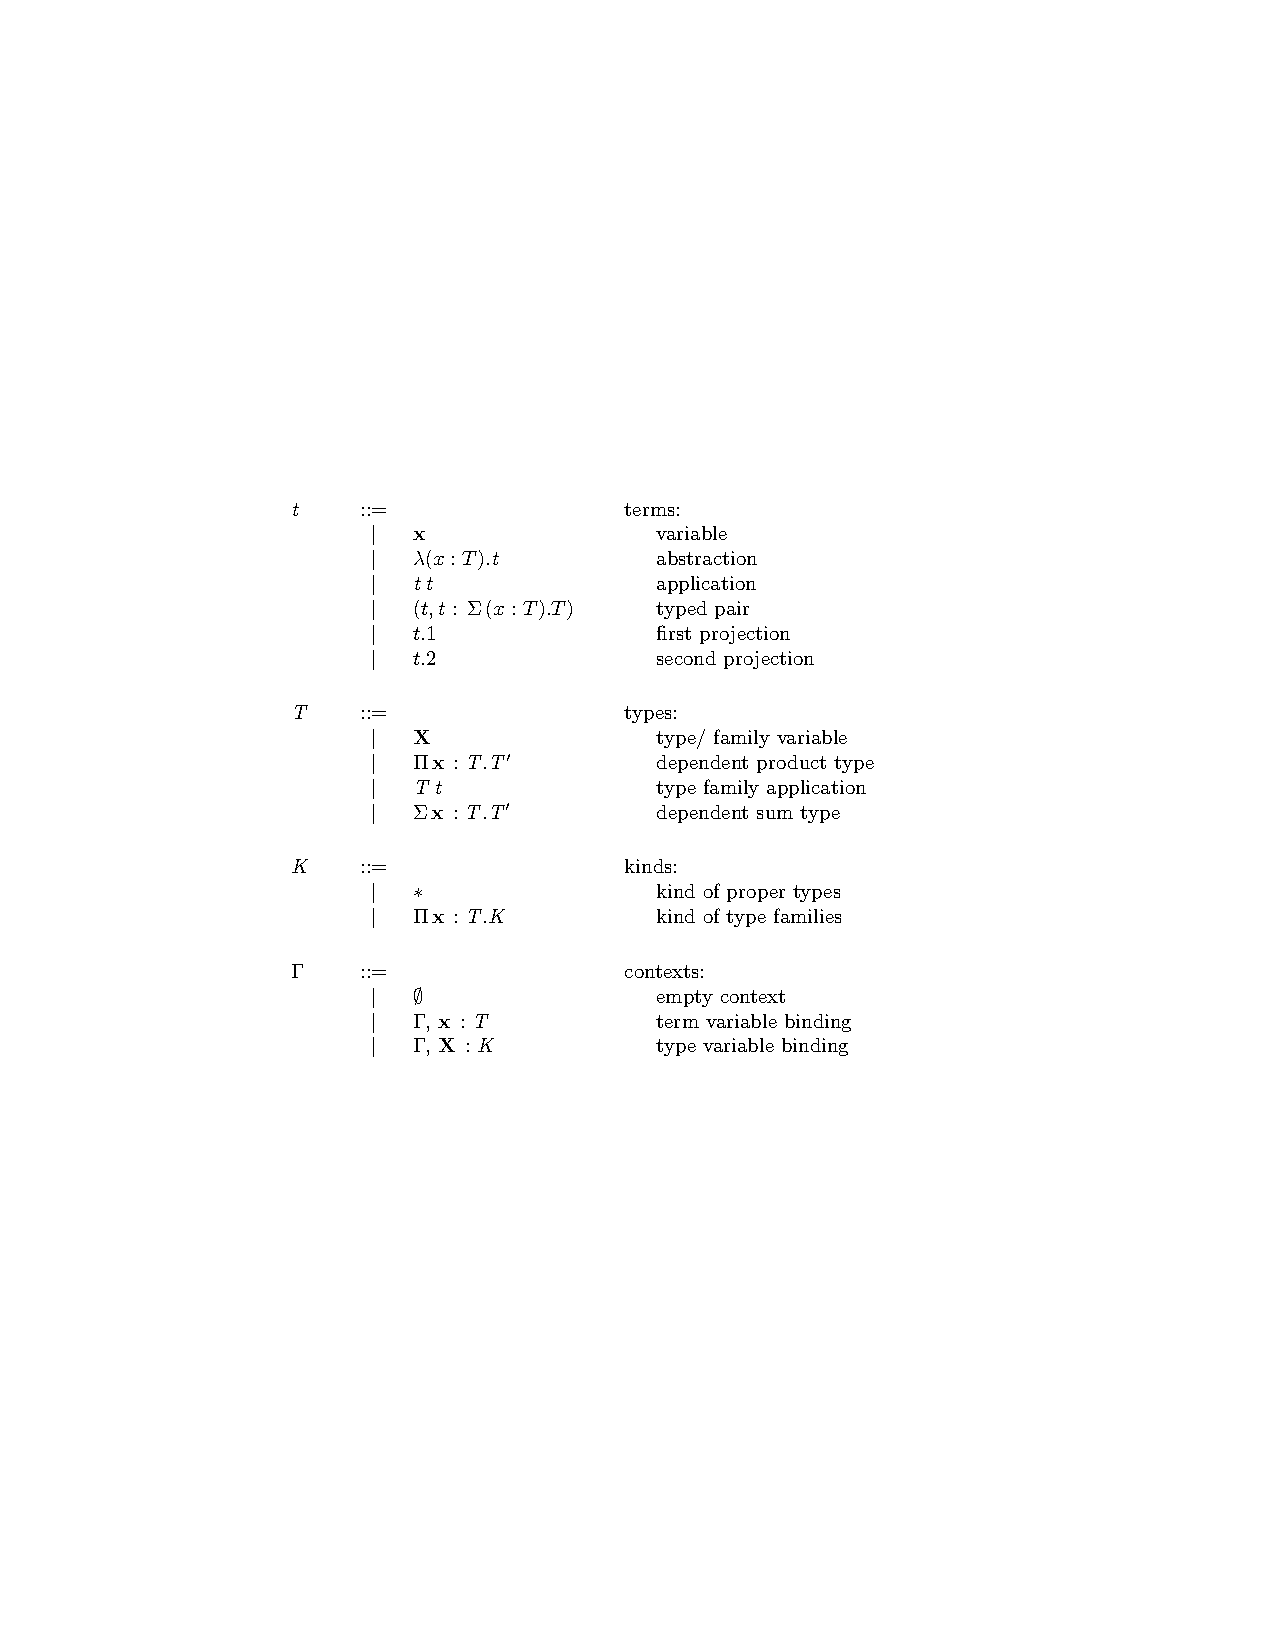
\includegraphics[scale=0.9]{ott/dttFig.pdf}
\caption{Grammar for a dependently typed language with dependent sum types. Adapted from~\cite{pierce2005advanced}.}
\label{fig:dttGrammar}
}
\end{figure}
\begin{figure}
    \begin{proofrules}
        \[ x : T \in \context{\Gamma} \qquad \Gamma \vdash T : *
        \justifies
        \context{\Gamma} \vdash x : T 
        \]
        \[ \Gamma \vdash S : * \qquad \Gamma, x : S \vdash t : T 
        \justifies 
        \Gamma \vdash (\lambda x : S \cdot t) : \Pi x : S \cdot T 
        \]
        \[ \Gamma \vdash t_1 : \Pi x : S \cdot T \qquad \Gamma \vdash t_2 : S 
        \justifies 
        \Gamma \vdash t_1 t_2 : T[x \mapsto t_2] 
        \]
        \[ \Gamma \vdash t : T \qquad \Gamma \vdash T \equiv T^\prime : * 
        \justifies 
        \Gamma \vdash t : T^\prime 
        \]
        \[ \Gamma \vdash \Sigma x : S \cdot T : * \qquad 
            \Gamma \vdash t_1 : S \qquad  \Gamma \vdash t_2 : T[x \mapsto t_1] 
        \justifies 
        \Gamma \vdash (t_1, t_2) : \Sigma x : S \cdot T 
        \] 
        \[ \Gamma \vdash t : \Sigma x : S \cdot T 
        \justifies 
        \Gamma \vdash t.1 : S 
        \]
        \[ \Gamma \vdash t : \Sigma x : S \cdot T 
        \justifies 
        \Gamma \vdash t.2 : T[x \mapsto t.1] 
        \]
    \end{proofrules}
\caption{Typing rules for a dependently typed language with dependent sum types. Adapted from~\cite{pierce2005advanced}.}
\label{fig:dtt-w-sigma}
\end{figure}

\paragraph{$\Sigma$-types.}
Types of dependent pairs, in which the type of the second element depends on value of the first one, are referred to as $\Sigma$-types. For example, 
%\sigmatype{n}{$\ \mathbb{N}\ $}{Vec A n}} 
\lstmath{$\Sigma\ $ n : $\ \mathbb{N}\ \cdot\ $ Vec A n} 
refers to the type of a pair that contains the value of \lstmath{n : $\;\mathbb{N}$} in the first position and a vector of length \lstmath{n} in the second one. 

\paragraph{Telescopes.}
The concept of $\Sigma$ types is generalized into that of \emph{telescopes}, or equivalently,  \lstmath{dependent-type records}~\cite{pollack2002dependently}. A telescope $\mathbb{T}$ is defined as 
\begin{equation}
\mathbb{T} \equiv [\text{x}_1 : \text{A}_1]
[\text{x}_2 : \text{A}_2(\text{x}_1)] \ ... \ 
[\text{x}_k : \text{A}_k(\text{x}_1,...,\text{x}_{\text{k}-1})]
\label{eq:telescope}
\end{equation} 
i.e. a sequence of typed name declarations where the type of later names can depend on earlier ones. 
The type \lstmath{Vec A n} represented as a telescope would be written as 
\lstmath{[A : Type][n :$\ \mathbb{N}$][Vec A n]}. 
%Another related concept is the packaging of definitions in a structure in which a definition depends on earlier ones. This is called a dependent record type, and is referred to as $\Sigma$-types. The types \lstmath{A} and \lstmath{P:A $\;\to\;$ Type} can be grouped is a dependent pair $\Sigma A P$. 

%\section{Curry Howard Correspondence}
%Also known as propositions-as-types and proofs-as-programs, the Curry-Howard correspondence relates constructive logics, like dependent type theory, to computer programs.\ednote{expand this}.  

\paragraph{Contexts.}
%\label{sec:background:context}
In logic, a proposition is true if it is an axiom or is derivable from other true propositions using inference rules. This is usually written as $\varphi_1 ... \varphi_n \vdash \psi$.  In categorical logic, instead of talking about propositions, one talks about contexts. \cite{handbook1993CategoricalLogic} defines a context as 
\begin{quote}
A context, $\Gamma$, is a finite list $[x_1 : \sigma_1, ... , x_n : \sigma_n]$ of (variable,sort) pairs, subject to the condition that $x_1, ... , x_n$ are distinct.  
\end{quote}
When using dependent types, the context becomes a telescope, where every type in the list can contain reference variables before it as described by Equation~\ref{eq:telescope}. The statement $\Gamma \vdash \psi$ means that the type judgement $\psi$ follows from the context $\Gamma$. The concatenation of two contexts $\Gamma_1$ and $\Gamma_2$ is noted by $\Gamma_1 ; \Gamma_2$.  
%\paragraph{The category of contexts}

%\todo{The ott grammar isn't showing up for some reason} 
%\documentclass{article}
\usepackage{supertabular}
\usepackage{dtt}
\begin{document}
   \begin{figure}
       \ottall
   \end{figure}
\end{document}



\section{Theories}
\label{sec:background:theory}
%The set of formulas is called the language of the logic. The language is defined syntactically; there is no notion of meaning or semantics in a  logic per se. 
A theory $\Gamma$ in some logic is defined as the tuple \lstmath{($\sort$,$\fsyms$,$\axioms$)} such that 
\begin{itemize}
\item $\sort$ is a set of sorts 
\item $\fsyms$ is a set of function symbols. 
\item $\axioms$ is the set of formulas that hold in $\Gamma$. 
\end{itemize}
The sorts in $\sort$ and the function symbols in $\fsyms$ constitute the language of the theory. 
The set $\axioms$ is closed under logical consequence and usually infinite. 
A \emph{theory presentation} of a theory $\Gamma$ includes a finite set of sorts, a finite set of function symbols, and a finite subset of $\axioms$ containing its generating axioms, i.e. axioms from which formulas that hold in $\Gamma$ can be derived using inference. 
Note that the same theory can have different theory presentations. 
In this work, as is traditionally the case, we use the term theory to refer to \emph{theory presentations}. 
%Most algebra text books would refer to the language of the theory presentation as the signature and would separate its two components, writing it as \lstmath{(S,F)}. They often do not use the term \lstmath{theory}, but refer to sigantures with specific properties that are satisfied by the algebras. The use of axiomatic theories as we define them here is, to the best of our knowledge, tied to using them in computerized systems as in Clear~\cite{Goguen1980}. 

\paragraph{Theories as Contexts}
With dependent types and the Curry-Howard correspondence in place, the distinction between the three components of an axiomatic theory, sorts, function symbols, and axioms, is not needed anymore. Instead, a theory is seen as a $\Sigma$-type, dependently-typed context, or a telescope as described by Equation~\ref{eq:telescope}. 
For example, the axiomatic formalization of \lstmath{Monoid} as a $\Sigma$ type is: 
%\begin{figure}
%\sigmatype{A}{Type}{\sigmatype{op}{(A $\to$ A $\to$ A)}{\sigmatype{e}{A}{Type}} }
%\end{figure}
%$\Sigma$ Type ($\lambda$ A $\to$ 
%$\Sigma$ A ($\lambda$ e $\to$ 
%$\Sigma$(A $\ \to\ $ A $\ \to\ $ A) ( $\lambda$ op $\to$ 
%$\Sigma$ ())))
\begin{lstlisting}[mathescape]
$\Sigma$ A : Type $\cdot$ 
 $\Sigma$ op : A $\;\to\;$ A $\;\to\;$ A $\cdot$ 
   $\Sigma$ e : A $\cdot$  
     $\Sigma$ lunit : {x : A} $\;\to\;$ op e x = x $\cdot$
       $\Sigma$ runit : {x : A} $\;\to\;$ op x e = x $\cdot$
         $\Sigma$ assoc : {x y z : A} $\;\to\;$ op x (op y z) = 
                                  op (op x y) z
\end{lstlisting} 
\noindent which can be describe as a telescope as:  
\begin{togcode} 
Monoid = [A : Set, op : A ~$\;\to\;$~ A ~$\;\to\;$~ A, e : A, 
          lunit : {x : A} ~$\;\to\;$~ op e x = x, 
          runit : {x : A} ~$\;\to\;$~ op x e = x, 
          assoc : {x y z : A} ~$\;\to\;$~ op x (op y z) = op (op x y) z] 
\end{togcode} 
\noindent This definition induces a context from which the type \lstmath{op e e = e} can be defined, which is noted as \lstmath{Monoid $\ \vdash\ $ triv : op e e = e}  

%The telescopic representation of a sort would be \lstmath{$\sort$:$\square$} where $\square$ is a kind defined in the type theory. A function symbol within a telescope is defined in terms of the type of its parameters. Propositions-as-types make it possible to present axioms as part of telescopes. is declared as $\sort : Type$. 
%Every declaration \lstmath{c:t} within the telescope is defined within a context \lstmath{$\Gamma$}. This is described as \lstmath{$\Gamma \vdash\;$ c:t}. 

%Theories in DTT are seen as contexts. This is how they are presented in~\cite{carette2018building} which forms the basis of this work. Therefore, we use the term context to also mean a theory in DTT. 

A theory presentation is well-typed if every declaration \lstmath{c:t} is well-typed given its context. The formation rules for theory presentations are given in Figure~\ref{fig:ctx}, where $\syms{\Gamma}$ refers to the list of symbols defined in the context $\Gamma$. 
$$ \syms{\context{\varnothing}} = \EmptyThy \qquad
\syms{\context{\Gamma}\ ;\ x : \sigma} = \syms{\context{\Gamma}} \cup \left\{ x \right\}
$$
\begin{figure}[ht]
    \begin{proofrules}
        \[ \ \justifies \varnothing \ \wfctx \]
        \[ \context{\Gamma}\ \wfctx \qquad \sigma \notin \syms{\context{\Gamma}}
        \qquad \context{\Gamma} \vdash \kappa : * \justifies
        (\context{\Gamma}\ ;\ \sigma : \kappa)\ \wfctx \]
        \[ \context{\Gamma}\ \wfctx \qquad x\notin \syms{\context{\Gamma}}
        \qquad \context{\Gamma} \vdash \sigma : \kappa : * \justifies
        (\context{\Gamma}\ ;\ x : \sigma)\ \wfctx \]
    \end{proofrules}
    \caption{Formation rules for contexts as given in~\cite{carette2018building}}
    \label{fig:ctx}
\end{figure}

\section{Theory Morphisms}
\label{sec:background:morphisms}
Morphisms are used to capture the structure of mathematics, by describing how theories are related to each other. In mathematical texts, a theorem proved for an arbitrary \lstmath{Monoid} can be used when considering an arbitrary \lstmath{Group} without extra work. Formally, this can be done if a meaning preserving morphism between \lstmath{Monoid} and \lstmath{Group} exists. The morphism specifies how results in \lstmath{Monoid} can be interpreted in \lstmath{Group}. 

A morphism $\arrow{[v]}{\Gamma}{\Delta}$ consist of a list of assignments $[v]$, a source theory \lstmath{$\Gamma$}, and a target theory \lstmath{$\Delta$}. 
$[v]$ assigns to every symbol\footnote{The symbols of a theory are the names of its declarations.} $x : \sigma$ in $\Gamma$ a term $r : \sigma[v]$ in $\Delta$. A term \lstmath{t} in the language of $\Gamma$ can be translated into a term \lstmath{t$^\prime$} in the language of $\Delta$ using substitution induced by the assignment $[v]$, such that  \lstmath{t$^\prime$ = t$[v]$}. Using the morphism 
\lstmath{[op $\ \mapsto\ $ + ; e $\ \mapsto\ $ 0] : Monoid $\;\to\;$ AdditiveMonoid}
we are able to interpret the expression \lstmath{(op e x)} in \lstmath{Monoid} as \lstmath{(+ 0 x)} in \lstmath{AdditiveMonoid} using substitution. 
%For example, a morphism from \lstmath{Monoid} to \lstmath{AdditiveMonoid} contains the assignments \lstmath{op to +} and \lstmath{e to 0} 

The formation rules for views are given in Figure~\ref{fig:views}. 
\begin{figure}[ht]
    \begin{proofrules}
        \[ \context{\Delta}\ \wfctx \justifies \view{}{\varnothing}{\Delta} \]
        \[ (\context{\Gamma}\ ;\ x : \sigma)\ \wfctx \qquad
        \view{v}{\Gamma}{\Delta} \qquad
        \context{\Delta} \vdash r : \substitution{\sigma}{v}{} \justifies
        \view{v,x \mapsto r}{(\context{\Gamma}\ ;\ x : \sigma)}{\context{\Delta}} \]
    \end{proofrules}
    \caption{Formation rules for morphisms as given in~\cite{carette2018building}}
    \label{fig:views}
\end{figure}

It is worth mentioning that the mapping is only a part of the morphism. A morphism consists of the source and destination theories as well as the mapping, i.e. the same substitution can induce different morphisms as the source and target are modified. 

Connecting theories have been known for a long time in logic~\cite{tarski1953undecidable, enderton1972mathematical} under the name \emph{theory interpretations}. The same name is used by IMPS~\cite{farmer1993imps, InterpIMPS1994}. Clear~\cite{Goguen1980}, OBJ, and their successors used the term \emph{morphisms}, maybe because of using category theory for semantics. The term \emph{view} has also been used to refer to the same concept by Maude, MathScheme, and MMT. In this work, we use the terms views and morphisms interchangeably. 

We distinguish between three types of morphisms.  

\subsection{Identity Morphism}
\label{sec:idmorph}
If $\arrow{[v]}{\Gamma}{\Delta}$ is an identity morphism, then $[v]$ maps every symbol $x \in \syms{\Gamma}$ to itself such that $x[v] = x$.
%This implies that $[v]$ is a bijection and that . 
While it is common to name source and target of identities with the same name, we do not do that here as $\Gamma$ and $\Delta$ are two different theory presentations. The identity between them means that symbols in $\Gamma$ are interpreted the same way in $\Delta$. 

Identity morphisms exist between two theories if the source is included verbatim in the destination, like in the case when describing a morphism from \lstmath{Monoid} to \lstmath{Group}. It is the simplest form of morphisms and allow transport of results without the need to perform substitution.  

\subsection{Embedding}
\label{sec:embedding}
If $\arrow{[v]}{\Gamma}{\Delta}$ is an embedding, then $[v]$ maps every symbol $x \in \syms{\Gamma}$ to a symbol $r \in \syms{\Delta}$, which is not necessarily itself. $[v]$ is an injective mapping, and therefore is a bijection onto its range. 

Consider for example, the following morphism from \verb|Magma| to \verb|AdditiveMagma|
\begin{equation*}\label{eq:additiveview}
\begin{tikzpicture}[node distance=9.0cm, auto,baseline=(current bounding box.center)]
\node (P) {$
    \begin{thyex}
    \thyrow{A}{\tmop{Type}}
    \thyrow{op}{A \rightarrow A \rightarrow A}
%    \thyrow{assoc_op}{\cdots}
    \end{thyex} $};
\node (B) [right of=P] {$
    \begin{thyex}
    \thyrow{A}{\tmop{Type}}
    \thyrow{+}{A \rightarrow A \rightarrow A}
%    \thyrow{assoc_+}{\cdots}
    \end{thyex} $};
\draw[->] (P) to node {$[A \mapsto\ A, 
    op \mapsto\ + ]$} (B);
\end{tikzpicture}
\end{equation*}
A term $t \in \Gamma$ is transported to $\Delta$ as $t[v]$, i.e.: by applying the substitution $[v]$ to the term $t$. 
So if \lstmath{$t =\ op\ x\ y$}, where $x$ and $y$ are terms of type $A$, then using the morphism above it is transported to $\Delta$ as $(+\ x\ y)$. 

We refer to an embedding morphism as $\widetilde{m}$, and therefore identity morphisms are referred to as $\widetilde{id}$. 

\subsection{General Morphism}
\label{sec:generalmorph}
A morphism in its general form as defined in the beginning of this section. 
%$\arrow{[v]}{\Gamma}{\Delta}$ is a general morphism if it maps symbols $x \in \syms{\Gamma}$ to terms $r \in \Delta$. 
An example is a morphism that flips a binary operation, i.e.: maps \lstmath{op x y} to \lstmath{op y x}
\begin{equation*}
\begin{tikzpicture}[node distance=9.0cm, auto,baseline=(current bounding box.center)]
\node (P) {$
    \begin{thyex}
    \thyrow{A}{\tmop{Type}}
    \thyrow{op}{A \rightarrow A \rightarrow A}
    \end{thyex} $};
\node (B) [right of=P] {$
    \begin{thyex}
    \thyrow{A}{\tmop{Type}}
    \thyrow{op}{A \rightarrow A \rightarrow A}
    \end{thyex} $};
\draw[->] (P) to node {$[A \mapsto\ A,
    op \mapsto\ \mathsf{flip}\ op]$} (B);
\end{tikzpicture}
\end{equation*}

%\section{Substitution}
%Morphisms acts on theories by substitution, i.e.: Given a morphism $[v] : \Gamma \to \Delta$, by performing the substitution of mappings in $[v]$ to symbols in $\Gamma$, we get the presentation $\Delta$. This substitution is written as $\Gamma[v]$. 
%Mappings acts on theories by substitution, i.e.: Given a list of assignments of terms to symbols $[x \mapsto y]$ and an expression e, a substitution replaces every free occurence of $x$ in the theory by y. 

\section{Theory Graph}\label{sec:background:theorygraph}
One way to organize theories is using theory graphs. A theory graph is a directed graph consisting of theories as nodes and morphisms as edges between them. It is helpful in managing large libraries~\cite{kohlhase2010towards}.

In systems that are based on categorical semantics, a theory graph is seen as a diagram in the category of theories and theory morphisms. Specware~\cite{Smith99} uses the keyword \emph{diagram} to build them. The work in~\cite{developmentGraph2000}, based on CASL, refer to them as \emph{development graphs}. 

Organizing a library as a theory graph leverages the structure of mathematics by relying on morphisms to connect the different concepts presented within the theories. Compare a library defining the graph leading to  \lstmath{Monoid} as in Figure~\ref{fig:cube_monoid} to one that defines it only in terms of its components, as in Section~\ref{sec:background:theory}. The theory graph one has more information which makes it more useful to library users. 


%\begin{figure}[h]
	\begin{tikzcd}[row sep=huge, column sep=scriptsize]
		&& & \verb|Pointed0| \arrow[dd,hook] & \\
		\verb|Carrier| \arrow[dd,hook] \arrow[rr,hook] & & \verb|Pointed| \arrow[ur,mapsto] & & \\ 
		& \verb|AddMagma| \arrow[rr,hook] \arrow[dd,hook]& & \verb|AddPointedMagma| 
		\arrow[rr,hook] 
		\arrow[dd,hook]& & 
		\verb|AddRightUnital|  \arrow[dd,hook]\\
		\verb|Magma| \arrow[ur,mapsto] \arrow[dd,hook]  & & 
		\verb|PointedMagma| \arrow[dd,hook] \arrow[ur,mapsto] \arrow[from=uu, crossing over] 
		\arrow[rr,hook,crossing over] \arrow[from=ll,hook, crossing over]
		& & \verb|RightUnital| \arrow[ur,mapsto] \\ 
		& \verb|AddSemigroup| \arrow[ddd,hook] & &\verb|AddLeftUnital| \arrow[rr,hook] &  & 
		\verb|AddUnital| \arrow[dddllll,hook] \\
		\verb|Semigroup|  \arrow[ddd,hook] \arrow[ur,mapsto]&  & \verb|LeftUnital| 
		\arrow[ur,mapsto] 
		\arrow[rr,hook,crossing over] &  & \verb|Unital| \arrow[dddllll,hook,crossing 
		over]\arrow[ur,mapsto] 
		\arrow[from=uu,hook,crossing over]& \\ 
		&&&& \\ 
		&  \verb|AddMonoid| &  &&\\ 
	 \verb|Monoid|  \arrow[ur,mapsto] && &&
	\end{tikzcd}
	\caption{Defining Monoid using tiny theories}
	\label{fig:cube_monoid}
%\end{figure}	

Theory graphs also makes it possible to modularize a formalization by adding definitions or proving theorems within smaller modules (theories). Definitions and theorems are then made available to different other theories by transporting them via morphisms. 

Here we discuss two strategies for decomposing theories; little and tiny theories.  

%By comparing the theory graph in Figure~\ref{fig:cube_monoid} with a definition of \lstmath{Monoid} in terms of its declarations shows how using a graph to define \lstmath{Monoid} leverages i
  
%Theory graphs leverage the structure of mathematics by relying on morphisms to connect the different concepts presented within the theories. 
%This way it is possible to add definitions and proof theorems within one theory 
%Therefore, it becomes possible to decompose definitions and proofs to pieces of knowledge into smaller contexts and perform reasoning within these contexts. In cases when this knowledge is needed in a different context, then transport them to different ones when needed. we are able to decompose the development of theories. Having morphisms also facilitates the transportation of results between theories. 

\subsection{Little Theories}
The little theories approach is introduced in~\cite{LittleTheories}. The idea is to ensure that if a statement \lstmath{s} is proven in context \lstmath{$\Gamma$}, then every statement in \lstmath{$\Gamma$} is required to prove \lstmath{s}. In this case, we say \lstmath{$\Gamma$} is the \emph{minimal axiomatization} needed to prove \lstmath{s}. This implies that theorems are proved in different contexts based on the amount of structure needed to prove them. In contrast, the big theory approach would use a small set of big theories for proving all results\footnote{Or a medium-sized set of medium-sized theories}. 

Using little theories increases the ability to reuse results. For example, if the theorem \lstmath{op e e = e} is proven in the theory \lstmath{Unital}, it can be transported to all theories that are connected to \lstmath{Unital} via morphisms, like \lstmath{Monoid}. On the other hand, if it is proven in the theory \lstmath{Group}, it cannot be transported to \lstmath{Monoid}, because all declarations in \lstmath{Group} becomes part of the context for proving the theorem.  
%to a less number of theories under the assumption that \lstmath{Group} is defined from \lstmath{Unital} using a series of extensions. 
%Results proven in the theory \lstmath{$\Gamma$} can be transported to all theories \lstmath{$\Delta$} whenever a morphism $m : \Gamma \to \Delta$ exists. 
% increasing usability and reducing redundancy when dealing with formal systems.  

\subsection{Tiny Theories}
\label{sec:background:tinytheories}
Tiny theories is a refinement of little theories. When building up a theory hierarchy in tiny theories style, only one new piece of information is added at a time~\cite{mathscheme2011experiments}. To make this clear, let us consider a library that has the theories \lstmath{PointedMagma} and \lstmath{Unital} defined as follows. \\
\begin{tabular}{p{6cm} p{7cm}}
\begin{lstlisting}[mathescape, basicstyle=\footnotesize]
theory PointedMagma = { 
  A : Type 
  e : A 
  op : A $\to$ A $\to$ A }
\end{lstlisting}
&
\begin{lstlisting}[mathescape, basicstyle=\footnotesize]
theory Unital = {
  A : Type 
  e : A 
  op : A $\to$ A $\to$ A 
  lunit : {x : A} $\to$ op e x = x
  runit : {x : A} $\to$ op x e = x   }   
\end{lstlisting}
\end{tabular}

Defining \lstmath{Unital} this way overlooks that in some cases one might want to define a theory to describe structures with a carrier and a binary operation on it that has only a right unit, like a theory with Integers as carrier and subtraction as the only binary operation. 
One will then need to add a new theory that is similar to \lstmath{Unital} without the \lstmath{lunit} declaration. Theorems proved in the context of \lstmath{Unital} cannot be used, even if they only depends on \lstmath{runit}. 

Using tiny theories, one would first define a \lstmath{LeftUnital} theory adding the \lstmath{lunit} axiom to \lstmath{PointedMagma}, a \lstmath{RightUnital} theory adding \lstmath{runit} axiom, and the theory of \lstmath{Unital} would be connected to both \lstmath{LeftUnital} and \lstmath{RightUnital}, creating more connections and therefore, allowing more reuse of results. Systematically using tiny theories to develop a large library leads to the need for support to diamond structures, which we discuss in Chapter~\ref{ch:library} based on the work in \cite{carette2018building}.  

\section[Category Theory]{Category Theory\footnote{This section is based on~\cite{pierce1990taste}.}}
\label{sec:categoryTh}
Category theory is a foundational framework, like set and type theory, that is abstract and structured enough to allow hidden commonalities of concepts to emerge. 

While set theory has elements of sets as the main concept, category theory is built around the concept of morphisms. The source and target of a morphism are objects in the category. Category theory is not concerned with the internal structure of the objects, but rather by how they relate to other objects. 

A category $\mathcal{C}$ consists of 
\begin{itemize}
\item A collection of objects, $\syms{\mathcal{C}}$
\item For any two objects, a collection of morphisms between them. A morphism between objects $\Gamma$ and $\Delta$ is presented as $u : \Gamma \to \Delta$.  
\item Operations assigning to every morphism its domain and codomain 
\item A composition function $\cdot$ assigning to each pair of morphisms  $u : \Gamma \to \Delta$ and $v : \Delta \to \Phi$, a morphism $v \cdot u : \Gamma \to \Phi$, such that for any arrow $w : \Phi \to \Omega$
\[ w \cdot (v \cdot u) = (w \cdot v) \cdot u \]
i.e. ($\cdot$) is associative. 
\item For every object $\Gamma$ in $\mathcal{C}$, an identity morphism $id_\Gamma : \Gamma \to \Gamma$, such that for $u : \Gamma \to \Delta$ 
\[ id_\Gamma \cdot u = u \cdot id_\Delta = u \]
i.e. $id_\Gamma$ is a left unit for ($\cdot$) and $id_\Delta$ is a right unit. 
\end{itemize}

A diagram in a category $\mathcal{C}$ is a graph homomorphism between collection of vertices and directed edges (the shape of the diagram) to objects and morphisms of $\mathcal{C}$. 
%Consistent labelling means that arrows of the category are represented by a directed edges whose source and target nodes have the same labels as the the objects of the category. 
% where by "consistency" we mean that if an edge in the diagram is labelled with the arrow f and f has domain A and codomain B, then the endpoints of this edge must be labelled with A and B. 
Finite categories can be represented diagrammatically as in Figure~\ref{fig:diagram}. 
\begin{figure}
\centering{
\begin{tikzcd}
 & \Gamma \arrow[loop] \arrow[dr,"k"]& \\
\Delta \arrow[loop left] \arrow[rr,"i"] \arrow[ur,"j"] & & \Phi \arrow[loop right] 
\end{tikzcd}}
\caption{A diagrammatic representation of a category}
\label{fig:diagram}
\end{figure}
A diagram is said to commute if for every pair of vertices, $\Gamma$ and $\Delta$, all paths from $\Gamma$ to $\Delta$ are equal, i.e.: compose to the same arrow. 

In the following we introduce two concepts related to categories that we use in Chapter~\ref{ch:library}. These are pushouts and colimits. \cite{nlab:colimit} gives an intuition of what a colimit is as 
\begin{quote}
``The intuitive general idea of a colimit is that it defines an object obtained by sewing together the objects of the diagram, according to the instructions given by the morphisms of the diagram"
\end{quote}
A pushout is a special case of a colimit. In~\cite{nlab:pushout}, it is mentioned that 
\begin{quote}
``A pushout is the colimit of the diagram 
\begin{tikzcd} 
\bullet & \bullet \arrow[l] \arrow[r] & \bullet
\end{tikzcd}"
\end{quote}
The formal definitions of the two constructions are given as follows: 

\paragraph{Colimits.}
Colimits are defined in terms of cocones. The definitions we present here are adapted from~\cite{sannella2012foundations}. 

A cocone over a diagram $D$ is an object $\Phi$ and a family of morphisms $u_0 : \Delta_0 \to \Phi, ..., u_{n} : \Delta_{n} \to \Phi$, 
where $\Delta_0\ ...\ \Delta_{n}$ are the objects in $D$, such that for every morphism $v : \Delta_i \to \Delta_j$ in $D$: $u_j \cdot v = u_i$, i.e. the following diagram commutes 
\begin{tikzcd} 
& \Phi & \\ 
\Delta_i \arrow[ur,"u_i"] \arrow[rr,"v"] & & \Delta_j \arrow[ul,"u_j"] 
\end{tikzcd}.
The notation used to describe cocones is 
$\langle u_i : \Phi \to \Delta_i \rangle_{i\leq n}$.

The colimit of a diagram is a cocone  
$\langle u_i : \Phi \to \Delta_i \rangle_{i\leq n}$ such that for any cocone 
$\langle u_i^{\prime} : \Phi^{\prime} \to \Phi \rangle_{i\leq n}$ there is a unique morphism $v : \Phi \to \Phi^\prime$ such that for every $u_i$, the following diagram commutes 
\begin{tikzcd} 
\Phi \arrow[ rr,dashed, "v"] && \Phi^\prime \\ 
& \Delta_i \arrow[ul,"u_i"] \arrow [ur," u_i^{\prime}"] & 
\end{tikzcd} 

\paragraph{Pushouts.}
The pushout is the colimit of a diagram $D$ that has exactly $3$ objects and $2$ morphisms. The morphisms need to have the same source. For a pair of morphisms $u_1 : \Gamma \to \Delta_1$ and $u_2 : \Gamma \to \Delta_2$, the pushout is an object $\Phi$ and a pair of morphisms $v_1 : \Delta_1 \to \Phi$ and $v_2 : \Delta_2 \to \Phi$ such that 
\begin{itemize}
\item $v_1 \cdot u_1 = v_2 \cdot u_2 $
\item for morphisms $w_1 : \Delta_1 \to \Omega$ and $w_2 : \Delta_2 \to \Omega$, there is a unique $w : \Phi \to \Omega$, such that 
\begin{itemize}
\item $w \cdot v_1 = w_1$
\item $w \cdot v_2 = w_2$
\item $w_1 \cdot u_1 = w_2 \cdot u_2$ 
\end{itemize}

\end{itemize}
The definition of the pushout is illustrated in Figure~\ref{fig:pushoutDef}. 
\begin{figure}
\centering{
\begin{tikzcd} 
\Gamma \arrow["u_1",d] \arrow["u_2",rr]& & \Delta_2 \arrow["v_2",d] \arrow["w_2",rdd, bend left] \\
\Delta_1 \arrow["v_1",rr] \arrow["w_1",rrrd, bend right]& & \Phi \arrow["w",dashed, rd] \\ 
& & & \Omega
\end{tikzcd}} 
\caption{Diagram illustrating the definition of a pushout}
\label{fig:pushoutDef}
\end{figure}

\begin{comment} 
\paragraph{Category of Theory Presentations}
Consider the category $\mathbb{P}$ of theory presentations as objects connected via morphisms. The theories \lstmath{Semigroup(SG)}, \lstmath{CommutativeMagma(CM)}, \lstmath{IdempotentMagma(IM)}, \lstmath{LeftDistributiveMagma(LDM)}, \lstmath{RightDistributiveMagma(RDM)}, 
\lstmath{LeftCancellativeMagma(LCM)}, and \lstmath{RightCancellativeMagma(RCM)}. The morphism between \lstmath{Magma = (A, op)} and any of those theories is the identity, as described in Section~\ref{sec:idmorph}. This leads to the following diagram: 

\adjustbox{scale=1.0,center}{
\begin{tikzcd} 
& & & \verb|Magma| \arrow[drrr,hook] \arrow[drr,hook] \arrow[dr,hook] \arrow[d,hook] 
  \arrow[dlll,hook] \arrow[dll,hook] \arrow[dl,hook]  & & & \\
\verb|LDM| &  \verb|SG| & \verb|RDM| &  \verb|CM| & \verb|LCM| & \verb|IM| & \verb|RCM|  \\ 
&&& \Xi &&& 
\end{tikzcd}
}

The colimit of this diagram is a theory with a carrier \lstmath{A} and one binary operation \lstmath{op} that has the properties described by the axioms in the theories connected to \lstmath{Magma}. Along with this theory are identity morphisms from all the theories in the above diagram to the colimit theory 
\end{comment} 

\section{Relational Interpretation}
\label{sec:background:relInterp} 
%A proof by logical relations proves some property $P$ of all closed terms of type $A$ by induction on types, i.e.: prove $P$ for all terms of type $A$, then prove it for terms of type $A \to A$, then terms of type $(A \to A) \to (A \to A)$

%A program consisting of a type and operations on that type can be seen as a theory. 
%When proving properties about programs, one often want to talk about structure-preserving relations between them, like equivalence. 

%Logical relations is a proof method that prove properties of programming languages. 

The relational interpretation of an algebraic structure is a generalization of its homomorphism~\cite{reynolds1983types} that defines a 
structure-preserving relation between carriers of its algebras. For example the relational interpretation between two monoid algebras $M_1 = (A_1,op_1,e_1,...)$ and $M_2 = (A_2,op_2,e_2,...)$ is a relation $interp : A_1 \to A_2$ such that: 
\begin{align*}
interp\ e_1\ e_2 &  \\
interp\ x_1\ x_2\ &\wedge\ interp\ y_1\ y_2\ \rightarrow\ interp\ (op\ x_1\ y_1)\ (op\ x_2\ y_2)  
\end{align*}
%We give a more generic \ref{sec:toBeGenerated}. 

%interp\ e_1\ e_2 \\
%interp\ x_1\ x_2\ \wedge\ interp\ y_1\ y_2\ \rightarrow\ interp\ (op\ x_1\ y_1)\ (op\ x_2\ y_2)  
%\end{eqnarray*} 

Relational interpretations are mainly applied to models of type theories. It has been used in~\cite{reynolds1983types} to develop the abstraction theorem that connects meanings of expressions under different assignments and in~\cite{parametricPoly93} to explain parameteric polymorphism. They have been applied to deduce theorems that apply to functions, given their polymorphic type~\cite{wadler1989theorems, algehed2020dynamic}. 
%Other applications include proving strong normalization, type safety, or equivalence of type systems~\cite{skorstengaard2019introduction}. 
They are used extensively when working on the semantics of programming languages, often refered to as \emph{logical relations}~\cite{crary2005logical}. Supporting proofs of logical relations has been considered a benchmark for theorem provers in the revised POPLmark challenge~\cite{poplmark2019}.  


%Relational interpretation is a concept used when reasoning about the semantics of prograamming languages. The algebraic interpretation of types views types and their related operations as 
%t is a generlization of the concept of homomorphisms between provides a syntactic translation 

%are used for reasoning about properties of programs, like type safety and equivelance of programs. 

%A logical relation is used to prove properties of programming languages. 
%Relational interpretation is a concept used when reasoning about the semantics of programming languages. It is used to 

\section{Multi-Stage Programming}
\label{sec:background:msp}
Meta-programming is the practice of writing \emph{meta} programs that manipulate \emph{object} programs~\cite{sheard2001Challenges, sheard2002TH,metaProg2019Survey}. Meta and object programs can be in the same or different languages. Generative programming is one form of meta-programming in which the meta-program compiles into a program of the object language. Therefore, the process of running the meta-program involves at least two stages, compile and run-time. 

The meta program might need to refer to code in the object language, like in the case of making a call to a predefined function in the object language. In this case, the meta program is deferring the evaluation of this code to a \lstmath{later} stage. 
Also, a meta program might need to evaluate a meta or object language expression that results in an object code. In this case, the expression is evaluated in the \lstmath{current} stage. 

In our implementation, we define two stages \lstmath{s0} and \lstmath{s1}. 
\begin{togcode}
data Stage : Set where
  s0 : Stage
  s1 : Stage
\end{togcode} 

Staging an expression means adding annotation to its components indicating which stage it should be evaluated in, 
\lstmath{Now} or \lstmath{Later}. 
\begin{togcode} 
data Staged (A : Set) : Set where
  Now : A -> Staged A
  Later : Comp A s1 -> Staged A
\end{togcode} 
Annotating an expression of type \lstmath{A} with the \lstmath{Now} constructor indicates that it will be evaluated in the current stage and a value of type \lstmath{A} is promised to exist. On the other hand, if the evaluation is deferred to \lstmath{Later}, then the expression will have the type \lstmath{Comp}, for computation. 
\begin{togcode} 
data Comp (A : Set) (s : Stage) : Set where
  Computation : Choice -> CodeRep A s -> Comp A s
\end{togcode} 
Computations encapsulate quoted fragments of code. The \lstmath{CodeRep} function assigns a stage \lstmath{s0} or \lstmath{s1} to the expression. 
\begin{togcode} 
data Wrap (A : Set) : Set where
  Q : A -> Wrap A
CodeRep : (A : Set) (s : Stage) -> Set
  CodeRep A s0 = A
  CodeRep A s1 = Wrap (CodeRep A s0)
\end{togcode} 
We also add a flag indicating whether the quoted code represents an expression (\lstmath{Expr}) or a literal, a constant or a variable (\lstmath{Atom}).  
\begin{togcode} 
data Choice : Set where
  Expr : Choice
  Atom : Choice
\end{togcode} 

Staging has $3$ main applications; generating well-typed code as in \mbox{MetaOcaml}~\cite{taha1999multi}, removing abstraction overhead introduced by generic programming~\cite{yallop2016StagingGeneric, carette2011mspFunctorsMonads, carette2011generative}, and developing domain specific languages~\cite{sheard2000stagingDSL}. MetaOcaml and Haskell templates provide staging constructs under the names \emph{quote} and \emph{eval} instead of \emph{Now} and \emph{Later}. In logical reasoning the same ideas are used for reflection, as in~\cite{farmer2013quoteEval}.  


%MSP gives the developers of the meta program the control over it by annotating which pieces can be evaluated at runtime\ednote{better writing}.  
%Writing program generators typically involve multiple stages; generation, compilation, and runtime stage. 
%MSP is a technique for managing code generation across different stages until execution. to provide annotations for the generator 

%\section{Finally Tagless}
%\label{sec:background:tagless}
%While staging is useful in so many ways, it introduces the overhead of dealing with the tags to \lstmath{Now} and \lstmath{Later}, or \lstmath{quote} and \lstmath{eval}. The finally tagless approach aim to remove this tagging overhead by encoding the object language as functions within a class, instead of constructors of a datatype. For example, the language of monoid would be represented as a type by: 
